\documentclass[10pt, twocolumn]{article}

\begin{document}
    \title{Node Placement for \\ Wireless Sensor Mesh Networks}
	\author{James Williams \\
			Swansea University \\
			williamsjn@protonmail.com\\
			\and
			Alma Rahat \\
			Swansea University\\
			a.rahat@swansea.ac.uk\\}
% Hard code the date or allow the LaTeX compiler to fill it in whenever you recompile the document.
	\date{\today}
	\twocolumn[
		\begin{@twocolumnfalse}
		\maketitle
	
		\begin{abstract}
			Wireless sensor mesh networks (WMNs) are a modern network topology where the placement of nodes has a large effect on the performance of the network. We enumerate some of their uses, demonstrating their flexibility and broad range of utility. We then consider a scenario of placing nodes in a network where testing each configuration of placements is costly in terms of time and resources. Then through the lens of this node placement scenario We introduce several popular optimisation techniques, some which are novel and subject of active research. We compare these methods and show how they have been implemented in the produced software. Software that has been created is demonstrated, potential extensions to the software and some open questions are reviewed and then concluding remarks are given.
		\end{abstract}
	\end{@twocolumnfalse}
	]
	
	\section{Introduction}
	\label{sec:intro}
	
	Emerging in the last two decades, wireless mesh networks (WMNs) are a relatively recent development in the domain of wireless networks which aim to surpass the performance of earlier wireless network layouts such as WPANs and WLANs\cite{akyildiza47wireless}. WMNs consist of an interconnection of `nodes', each of which is a device equipped with a radio that can communicate with other devices within a certain distance of another device. The `mesh' in wireless mesh networks refers to an approach in network topology under which each of the devices connect to each other directly rather than having to wait for any centralised authority, though there may be sources of authority on certain matters. This topology allows for a great degree of flexibility but also adds significant complexity over more traditional topologies. 

	The applications of WMNs are numerous as they are, at their most generic level, just another way of organising a wireless network. Usage could span from consumer `internet of things' (IoT) devices within a home with only a single floor \cite{apte2018home} to specialised equipment that detects fires in hundreds of square kilometres of forests\cite{lloret2009wireless}\cite{jin2018evaluation}. As might be apparent the location and configuration of the individual nodes in wireless sensor mesh networks can have a large impact on the cost and performance of the network along almost every axis. Desired properties of the network such as speed or resistance to individual node failure will also impact node placement. This is an active research area\cite{younis2020placementsurvey}.

	
	\subsection{Motivations}
		\label{sec:intro_motivation} 
		
		In order for our research to remain focused in such a wide area of study, we have taken the example of node placement in an indoor museum and consider how we could optimise a hypothetical scenario in which a network engineer installing wireless nodes must measure the strength of connectivity of sensors to a collection of nodes through a series of predetermined tests. In the event that the results of the measurements are not acceptable, the nodes must be moved in order to increase the strength to an acceptable level. In addition to simply finding the ideal placement for nodes, constraints can complicate the process of placement such as adhering to fire safety code and more literal physical constraints (e.g. a node cannot be placed inside of a supporting column.)
	
	\subsubsection{Objective}
		\label{sec:intro_objective} 
		
		Deciding node placement for the scenario given above is difficult and also very time consuming. By utilising optimisation techniques we can minimise the number of tests and measurements that have to be taken and reach stronger configurations sooner. We have considered many optimisation techniques in the process of research, detailing their benefits and drawbacks and demonstrating this through data collected. Traditional techniques such as random search, simulated annealing and genetic algorithms have been considered alongside a more novel approach; Gaussian processes, a Bayesian modelling technique\cite{rahat2020bayesian}. This approach is driven by the data given in response to the predetermined tests. 

		We frequently revisit our specific node placement problem in order to demonstrate the effectiveness of an optimisation when applied to a real problem, but it is important to consider the breadth and depth of this problem and how each optimisation could be applied to not just this specific scenario. 
		
	\subsection{Overview}  
		\label{sec:intro_overview} 
		
		The rest of section \ref{sec:intro} is dedicated to the contributions of this document as well its structure. Section \ref{sec:problem} details the problem statement and a brief outline of potential solutions. Section \ref{sec:related_work} provides an overview of similar research and areas related to this work as well as its applications in industrial settings. Section \ref{sec:traditional} scrutinises the traditional optimisation techniques and section \ref{sec:bayesian} focuses on Bayesian optimisation. Section \ref{sec:comparison} compares the aforementioned optimisation techniques. Section \ref{sec:extensions} discusses the shortcomings of the current software and what might be improved in the future. In section \ref{sec:conclusion} the findings and products of this project are summarised.
	
	\subsection{Contributions} 
		\label{sec:intro_contribs} 
		
		The contributions of this dissertation are the following:
		
		\begin{description}	
		
			\item A software library for the optimising of 2D node placement
			
			This library is general enough to be used in any 2D node placement project and also easily modifiable to suit more specific needs.
			
			\item Software aiding the use of the optimisation library
			
			For users who do not have a great deal of programming skill, this software works out of the box to interface with the library in an easy to understand way.
			
			\item This document
						
			We review techniques and compare their usefulness in response to the growth of the number of dimensions and the complexity of the objective function (see chapter \ref{sec:problem}).
			
		\end{description}
	\section{Problem Statement}
	\label{sec:problem}
	The introduction details the specific troubles of node placement. This problem is sufficiently complex and so often repeated that it bears worth researching and developing software solutions for. During the course of our research we have developed software that enables the optimisation of placement of nodes given constraints both in terms of the time to generate the next candidate solution as well as finding an approximate global optimum configuration as quickly as possible.
	
	\subsection{Free Space Path Loss}
		\label{sec:problem_FSPL} 
		We can define the process by which we measure the free space path loss (FSPL) \cite{monebhurrun2019standard} of each node:
		\begin{equation}
			g(S_n, D)
		\end{equation}
		where $S_n$ is a source node $s \in S = (S_1, S_2, S_3, ..., S_n)$, $D$ is a list of destination nodes $d \in D = (D_1, D_2, D_3, ..., D_n)$. In some cases, $S = D$ and $S_n \in D$ as WMNs may seek to re-broadcast data through other nodes in order for the data to reach another point. Here, the global optimum is the minimum value as we want to minimise the FSPL.
		
		From the set of results that we generate by running the function $g$ over all the given nodes we find the layout $l = (S, D)$ from the set of all possible layouts $L$ of the nodes with the lowest average minimum FSPL. Mathematically, we are searching for the global minimizer of the objective function $g$:

		\begin{equation}
			l* = \underset{l \in L}{arg\: min}\; g(l)
		\end{equation}

		The set $L$ of all possible layouts can be extremely large and while each evaluation of $g$ takes linear time $O(n)$ in the size of $D$, the brute force approach to evaluating a single layout is quadratic $O(n^2)$, making a single large layout evaluation computationally expensive. By minimising the FSPL, we are maximising the connection strength and ability of the source node to access the destination nodes.
	\subsection{Broadness of the Problem}
		\label{sec:problem_broadness} 
		In practice this notation lacks detail on how we deal with the practical constraints of placing wireless nodes in a real building. For example, power may only be available in certain places, fire safety code will prevent us from placing sensors in certain locations. There are many ways of dealing with possible constraints. By publishing the code, we have given a great degree of control to other developers making use of the optimisation library so that they may introduce their own complex constraints based on outside sources of information. In turn the developer will have to engage on a deeper level with the library's code in order to extract the maximum utility from it. Keep in mind that the examples given above are not a reflection of limits that are be put in place by the optimisation library and that it is applicable in any environment, not just indoors. It could be used just as easily to optimise the placements of geo-stationary satellites in orbit of a planet as for placing sensors in a museum.
		
	\subsection{Working Towards a Solution}  
		\label{sec:problem_solution} 
		As we have referred to in section \ref{sec:intro_contribs}, part of this project's production is the creation of a general software library for optimising node placement. In the creation of this library we have examined various `traditional' optimisation techniques such as random search, genetic algorithms, simulated annealing as well as more novel techniques such as Gaussian processes. Each of these optimisation techniques can be easily be reused by another program that submits an equivalent objective function. This library is  primarily focused on ideal placement of vertices in two-dimensional space, with specific attention on minimising the number of iterations required to find an approximate global optimum.

		By benchmarking each of the optimisation techniques in their effectiveness in terms of the minimum number of operations required to achieve an acceptably low distance from the global optimum as well as time taken we aim show that both classic and novel optimisation techniques can provide significant improvements in minimising the time spent by engineers attempting to generate the ideal placement of wireless nodes.
	\section{Related Work and Industrial Applications}
	\label{sec:related_work}
	As an active research area, there is a great wealth of work solely focused on the optimisation of the placement of nodes as well as mesh networks, wireless or otherwise. Considering the hardware involved, the deployment of a wireless mesh network must consider the strength and configuration of the radios, its resistance to the elements of the environment it is placed in, the source of the power and its reliability as well as that level of reliability's effect on the choice on how data is stored. Depending on the requirements of the network, legal requirements might add further constraints such as a given amount of time logs and records must be kept for and the ability to verify the authenticity and accuracy \cite{gdpr} of those logs.

	This section details the various areas related to wireless mesh networks and the optimisation of their placement, both traditional and more novel approaches, including work done by other researchers with similar but distinct objectives. We also discuss the various ways in which industry might seek to apply these concepts.

	\subsection{Distributed Systems}
		\label{sec:related_work_distributed} 
		When we turn to the software involved we can observe that mesh networks are an example of distributed systems, another very active research area looking to tackle problems of distributed consensus \cite{lamport2019byzantine} \cite{paxos} \cite{raft}, node failure and parallel algorithms to name just a few. Each of these problems are difficult and solutions inherently involve some trade-off that must be made in line with the constraints and desired properties of the solution.

	\subsection{Extraplanetary Applications}
		\label{sec:related_work_spacex} 
		As covered in the introduction, wireless mesh networks are deeply flexible and have a wide number of possible applications\cite{akyildiza47wireless}. A very recent example of this is SpaceX's Starlink project which seeks to deploy 2,825 satellites. In addition to each of the satellites covering an individual area to provide a single intermediary between a user and a "gateway earth station" for satellite internet access, "The system will also employ optical inter-satellite links for seamless network management and continuity of service\cite{fccspacextechnicala}." Contained in this one sentence is a world of complexity with regards to implementation that takes advantage of cutting edge hardware and software research with heavy use of the research into areas such as distributed systems and radio equipment. As you may be able to guess from figure \ref{fig:spacex}, the placement of these nodes changes from moment to moment as the satellites orbit earth according to expected traffic.
		\begin{figure}[H]
		\centering
		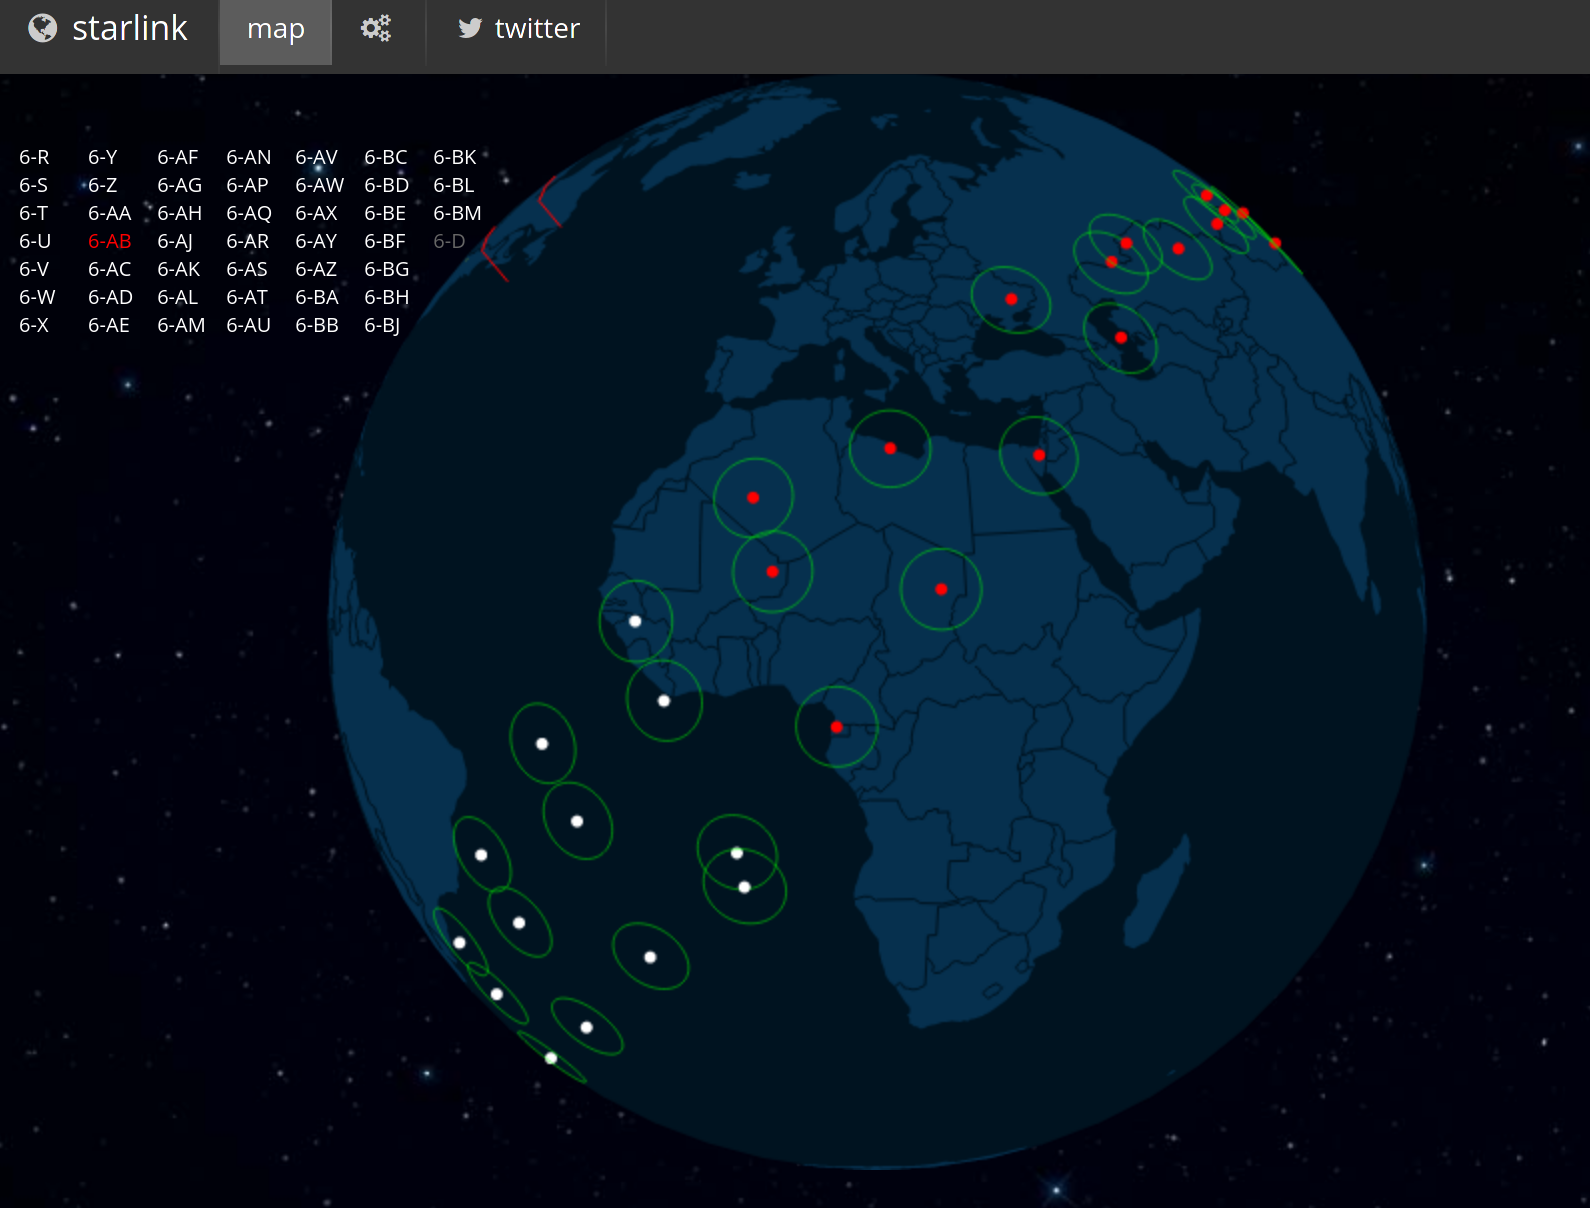
\includegraphics[scale=0.21]{graphics/spacex_map}
		\caption{SpaceX Starlink Satellite Map \cite{satellitemap}}
		\label{fig:spacex}
		\end{figure}
		
	\subsection{Optimisation}  
		\label{sec:related_work_optimisation} 
		Focusing solely on the subject of node placement in wireless mesh networks, there has been so much research that a survey of some of the many strategies and techniques in node placement exists\cite{younis2020placementsurvey}. This survey goes into detail concerning node distribution, deployment objectives, dynamic repositioning of nodes and existing open research problems. The impact of the desired properties such as primary objectives and constraints of the system on node placement is repeatedly highlighted and given its own column on multiple tables, making it clear that there is no `one size fits all' approach to node placement. 

		From this we can infer that if we wish to build software that evaluates the suitability of and optimises node placements in a generic way it is of vital importance that we allow for users of that software to provide their own constraints and objectives comprehensively. While there is a place for novice users with no ability to program making use of GUI software, utilising complex optimisation software will require the users to be programmers capable of providing functions to the library that we have developed in order for the software to accurately evaluate the suitability of a set of node placements according to their unique specifications.

		\subsubsection{Traditional Algorithms}
			\label{sec:related_work_traditional}
			Sharpening our focus still onto the optimisation of node placement we find a few common optimisations. The first one is random node distribution, which is covered in the aforementioned survey.\cite{younis2020placementsurvey} Many research papers already exist that have considered the use of random node distribution and evaluation\cite{wang2010coverage} according to given constraints and objectives. However some researchers go further than this naive optimisation approach, considering single and multi-objective genetic algorithms (MOGAs)\cite{zhang2017flexible}, greedy algorithms and cluster placement for enhanced performance\cite{bi2015node}. An important consideration is that MOGAs are more suited for `objective' functions with fast execution times, but not for those that are slow to compute. This is because genetic algorithms typically create a population of candidate solutions\cite{banzhaf1998genetic} the size of which is dependent on the nature of the problem but could well be in the thousands. As such, evaluating each of the population for an expensive algorithm for each generation quickly becomes computationally infeasible.

		\subsubsection{Bayesian Optimisation} 
			\label{sec:related_work_bayesian} 
			Bayesian optimisation is an approach to global optimisation that evaluates data as it is collected using a `sequential' design strategy\cite{movckus1975bayesian}. This strategy makes Bayesian optimisation uniquely suited to optimising computationally expensive `cost' functions,\cite{brochu2010tutorial} which are functions that take a range of values and return some real number, allowing that result to be compared with other results of other ranges of values. This methodology makes no assumption about the form or behaviour of the function, treating it as a `black box'.

			As of writing, we have not seen any evidence that the approach of Bayesian optimisation has been used or published and as such this research is novel in this way. Shahriari et al. discuss Bayesian optimisation at length in `Taking the Human Out of the Loop: A Review of Bayesian Optimization'\cite{shahriari2015taking}, laying out many of the possible and already existing applications of Bayesian optimisation as well as thorough psuedo-code implementations of a number of ways in which Bayesian optimisation can be implemented. `Acquisition' functions are also discussed which are used to find the exact query points that will best further guide the algorithm's understanding of the search space. More detail about Bayesian optimisation is given in chapter \ref{sec:bayesian}.
			\begin{figure}[H]
			\centering
			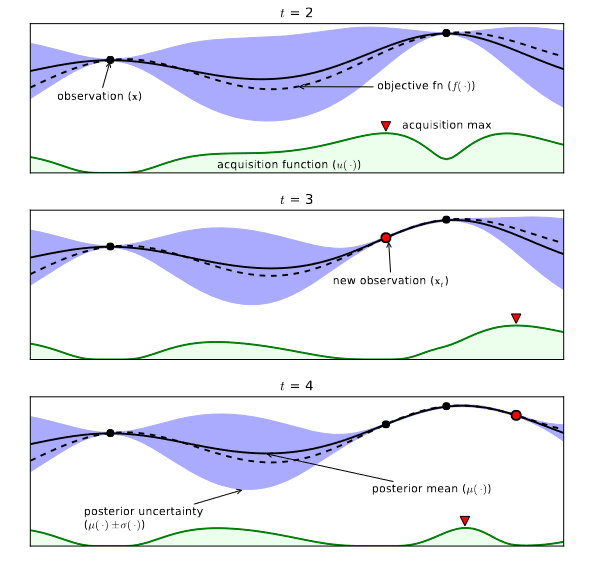
\includegraphics[scale=0.6]{graphics/bayesian_1d}
			\caption{Bayesian Optimisation on a toy one-dimensional problem. \cite{brochu2010tutorial}}
			\label{fig:bayesian_1d}
			\end{figure}
	\subsection{Industrial Applications}
		\label{sec:related_industrial}
		As we've discussed in section \ref{sec:problem_broadness}, there are a wide range of places industry might seek to apply the optimisation of wireless node placement. Internet-of-things devices are increasingly common in consumer and office environments \cite{evans2011internet}, all of these devices sharing the key characteristic of requiring strong and reliable access to a network in order to exchange information among each other and often with the outside world. Poor signal inhibits the advantages of these devices and so maximising signal ($\approx$ minimising distance) is of vital importance.

		In the example of Starlink, running network simulations and experiments long before the launch of the network will surely have taken place to plan traffic flows and measure the strength of the connection from the surface to satellites and satellite to satellite. The expense involved in launching such a network would preclude testing in a live environment. The placement of individual satellites would also heavily benefit from the optimisation of placement according to the required bandwidth at certain points in the day.

		On a different scale, office employees are increasingly using wireless devices instead of wired computers at fixed desks. Under these circumstances having strong connection coverage is important to ensure that employees attempting to access local and remote resources can do so efficiently. Planning the placement of nodes to optimise for coverage would be wise and not doing so would have a negative impact on employees.
	\section{Traditional Techniques}
	\label{sec:traditional}
	In the process of optimisation a single technique is applied repeatedly to produce a query for the objective function, which returns a result, and eventually a final solution is given. The number of repetitions of this process, its boundaries and constraints and whether it is seeking to minimise or maximise results from the objective function are all key but extraneous factors for the technique (or algorithm.) We consider these factors among others in which algorithm we use but they do not guide the core principles which are typically based on the trade off between exploration and exploitation.
	
	\subsection{Random Search}
		\label{sec:traditional_random} 
		The process of random search is strikingly simple. Given that we have an objective function we can query and we know its bounds, we simply generate random valid coordinates and query the function for as many iterations as are feasible or are allowed by the constraints of the problem.

		Random search is one of the exceptions to the above assertion that there is some balance to be struck between exploration and exploitation. One could choose to say that random search is pure exploration as it makes no decisions based on results previously gathered. This choice is naive and in highly dimensional problems is unlikely to yield any significant results in an environment where the objective function is computationally expensive. However, because it uses none of the previous results it is also embarrassingly parallel as no communication is needed between agents making decisions about which query to make next.
		
		Under certain circumstances random search may be an effective and appropriate way to query a search space but these circumstances are likely few and far between.
		
	\subsection{Genetic Algorithms}  
		\label{sec:traditional_genetic}
		Genetic algorithms are a class of optimisation algorithms that make use of the concept of natural selection\cite{darwin1909origin}, where solutions to the problem `evolve' through random mutation and inheritance from existing top candidate solutions. The application of concepts from the natural world in computer science is not new by any means. In \textit{I.---Computing Machinery and Intelligence} by A. M. Turing\cite{turing1950learning}, published in 1950, Turing talks about a machine's ability to learn through repetition of teaching and evaluation and this processes's parallels with evolution. In our example, we consider natural selection to be equivalent to the objective function evaluation and its result. 

		The basic flow of a genetic algorithm is as follows. First, a random population is created then evaluated and sorted according to the objective function's response to the decision variables. Then the process of crossing over and mutating the parents begins. According to predetermined probabilities, the  mutation for individual genes is carried out and the crossover of the parents is carried out. For example, a function with four dimensions would have parents with two nodes each (as each node has two coordiantes.) During crossover two children are created, one with the left node from the first parent and the right node from the second parent and another vice versa. Once the children are created, they are evaluated and the top `children' from the population are the input population for the next iteration.

		In our implementation, the `genes' are represented by the coordinates of the nodes to be placed. The parallels between individual nodes in a configuration and genes are quite apparent. As such, parents can pass genes onto their children in the form of entire nodes as both the X and Y coordinates are preserved. However the preservation of individual nodes that make up known good parents do not necessitate a better or even equivalent child; the same is true in biology. Perhaps some of the nodes of the children are simply repeated, reducing coverage and yielding a lower objective function response. Mutation is carried out by Gaussian mutation, which finds a middle point and then adds a random factor from a Gaussian (normal) distribution. In this way, genetic algorithms intelligently exploit known optimal parents but continue exploring by creating children and mutating them to add an element of random exploration as in the natural world.

		There are drawbacks to genetic algorithms. Genetic algorithms are not easily parallelisable and would require concurrent work to stop and results to be compiled every time a new generation was created. Additionally, genetic algorithms can often `converge'\cite{langdon2013foundations} earlier than ideal, ending the exploration phase, if one individual is significantly superior or `fitter' than its peers.

	\subsection{Simulated Annealing} 
		\label{sec:traditional_simulated_annealing} 
		Simulated annealing is another algorithm that makes use of past function evaluations to make decisions about the next query point. Taken from the concept of `annealing' in metallurgy (a domain of science concerning metals), this algorithm uses a cooling or `decay' curve that represents the preference for exploitation instead of exploration as the number of function evaluations increases. 

		We carry out the process of exploration through the choice of a new `neighbour' to the current state. The distance that the state can travel is bounded so that we only move so fast through the function space and give the algorithm adequate opportunity to explore each potential space. This bound can be tightened or widened in order to favour exploration or exploitation more explicitly. In multi-dimensional functions we apply a change to all dimensions. This does not mean that each individual dimension will necessarily move as the neighbour function may select this node to travel an insignificant distance (or potentially no distance at all.)
		
		In earlier evaluations a simulated annealing algorithm is more likely to accept a poorer solution as the next iteration's starting state for the sake of exploring the function space. In later evaluations this becomes increasingly unlikely to happen and instead only superior solutions are accepted as the new current state in the function space.
		
		This algorithm makes explicit the decision of exploration versus exploitation. As we have additional information from the exploration phase, we gain a greater degree of confidence about our understanding of the overall function space. Exploitation becomes increasingly attractive though the gains made from this are usually fairly minimal. To reflect this, in our implementation we use a `fast' cooling curve:
		\begin{equation}
			 t_k = \frac{t_i}{k}
		\end{equation}
		where $t_k$ is the temperature at the $k$th iteration and $t_i$ is the initial temperature. Despite its name, it is one of the slower decay curves. We chose an initial temperature of 5.5\cite{wright2010automating} so as to reduce the initial state's impact on the final result.

		Simulated annealing thrives in environments where it can make a large number of queries to the objective function in order to gain as much information as possible. However it can be slow to find optimums depending on the choice of decay curve and how neighbours are chosen. 
		
	\section{Bayesian Optimisation}
	\label{sec:bayesian}
	In environments where the `dimensionality' or the number of decision variables of the objective function (as seen in section \ref{sec:problem_FSPL}) is high, optimising the inputs can be intensive in both time and resources. In many circumstances there are hundreds or even thousands of these `free variables' such that even a team of humans could not hope to make smart decisions about the next point to query. Similarly, attempting to exhaustively evaluate the entire search space using an optimisation method such as grid search rapidly becomes infeasible with increasing dimensionality due to the time and other constraints of carrying out such a computation.

	Bayesian optimisation is an emerging optimisation method with a broad range of applicability. The optimisation of the parameters of optimisation algorithms, known as hyperparameter optimisation, is just one example of Bayesian optimisation's potential uses. This means we could potentially make use of our Bayesian optimiser to optimise our traditional algorithms if we felt so inclined. Other uses include machine learning, environmental monitoring and big data\cite{shahriari2015taking}.
	
	\subsection{A Brief, Technical Overview}
		\label{sec:bayesian_overview} 
		Bayesian optimisation is a novel approach to optimisation that makes use of Gaussian processes. This approach takes a sample of existing function evaluations and trains a Gaussian model on these input evaluation pairs. The inputs to these function evaluations are chosen through `latin hypercube sampling'\cite{deutsch2012lhs}. Latin hypercube sampling is a method of ensuring better random coverage of a highly dimensional space by dividing the number of query points into intervals and placing those intervals at sufficient distance from the other points. The Bayesian model creates a predictive distribution formed by knowledge we have about the objective function given from the sample of existing function evaluation results and their inputs.

		The foundation of this process is Bayes' theorem.
		\begin{equation}
			p(A | B) = \frac{p(B | A) p(A)}{p(B)}
		\end{equation}
		This statement means that the probability of A occurring given that B is true ($P(A | B)$) is equal to the probability of B if A is true ($P(B | A)$) multiplied by the probability of A ($P(A)$) divided by the probability of B ($P(B)$). As it applies to our optimisation use, B is the known data the model has been trained on and A is an unobserved quantity.
		
	\subsection{Surrogate/Acquisition Function}
		\label{sec:bayesian_surrogate}
		The Gaussian process regressor (GPR) gives us an `acquisition' (or surrogate) function which is not the objective function itself, but rather an expressed belief about the probability of improvement if we choose to sample this space.

		We use a method called `expected improvement' as our decision criterion in order to derive the likelihood of improvement from the result of the surrogate function. Expected improvement is not the only decision criterion we can use to compute the best next point to sample given the output of the GPR, but it is the one that has been implemented for this project. As seen in \ref{fig:bayesian_1d}, the likelihood of improvement approaches zero as the acquisition function heads towards a sampled point. In tandem with this, the degree of uncertainty about the function decreases as we approach a sampled point. This figure also accurately expresses the desire to exploit around (but not exactly at) the current optimum point compared to other points in the function space. Unlike previous algorithms we have considered, new information gained from sampling a point can intelligently re-focus the algorithm on exploration of the function space; each iteration is not simply one step closer to exploitation.

		Of course, we've effectively moved from one function we want to optimise to another function we, simlarly, want to optimise. This transition is not fruitless, as with an expensive objective function the surrogate function will allow us to sample without incurring this expense. If we have constraints related to how many times we can sample the objective function or time itself, this function speeds up the process greatly.

	\subsubsection{Simulated Annealing for the Optimisation of the Surrogate Function}  
		\label{sec:bayesian_annealing}
		As we discussed in section \ref{sec:traditional_simulated_annealing}, simulated annealing is an effective method of sampling the function space for an optimum based on concepts borrowed from metallurgy. In order to sample this new function we need a method that is not Bayesian optimisation, otherwise we encounter a problem of infinite recursion.

		Simulated annealing is a strong candidate for the optimisation of the surrogate function for the reasons discussed in section \ref{sec:traditional_simulated_annealing} and as it intelligently samples the function space and can be tweaked to favour exploration or exploitation according to the needs of the user.
	
	\subsection{Applicability to Node Placement} 
		\label{sec:bayesian_applicability} 
		Evaluating the suitability of a node placement configuration is difficult and depends on the desired characteristics of the network. These evaluations can span anywhere from simple implementations (such as our free space path loss implementation as seen in section \ref{sec:problem_FSPL}) to complex simulations that may take hours to complete. Additionally the dimensionality of the problem becomes increasingly complex with each additional node. In two-dimensional space each node has two dimensions, whilst in three-dimensional space they have three. The consequences of this are that a relatively simple network configuration problem with only two nodes to place can be anywhere between four and six-dimensional problems. With every added dimension the problem space becomes exponentially larger. As can be derived from the above, Bayesian optimisation is well suited to problems where the objective function is computationally expensive with high numbers of dimensions\cite{shahriari2015taking}. 

		
	\section{Comparison}
	\label{sec:comparison}
	In order to assert that one optimisation technique is superior to another, we will need to employ some degree of statistical analysis. This is because, among other reasons, all of the optimisation techniques concerned are non-deterministic. This means that on individual runs each optimisation technique may yield vastly different results. Some of these may be superior to others more often than not and so we quantify this in order to be more certain. See page over.
	\subsection{Improvement Performance Profiles}
		\label{sec:comparison_improvement_profile} 
		To graphically demonstrate the performance of the optimisers against each other, we recorded their best found result at each step of the iteration with the environment variables. Some translation was done for comparison of results where there was not a strict relationship between an iteration and objective function calls.
		\begin{figure}[H]
		\centering
		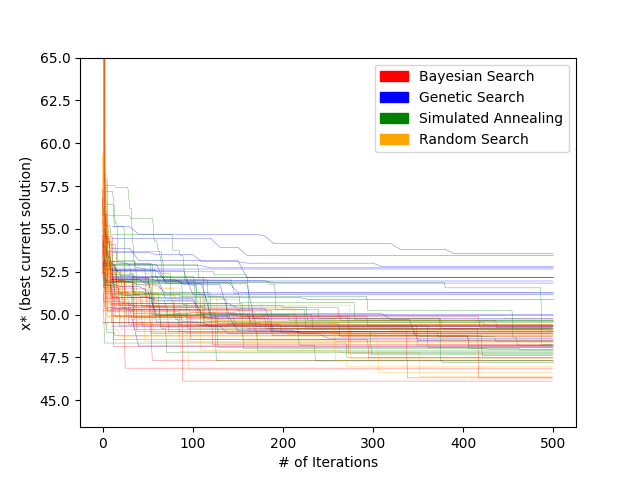
\includegraphics[scale=0.75]{graphics/performance}
		\caption{Performance of Bayesian Search, Genetic Search, Simulated Annealing and Random Search compared over 25 runs of 500 iterations.}
		\end{figure}
	\subsection{Mann-Whitney U Test}  
		\label{sec:comparison_mann-whitney} 
		The Mann-Whitney U test is a test of the null hypothesis that for a random selection of values (A and B) from two discrete populations, the likelihood of A being greater than B is equal to B being greater than A. This test produces a `U statistic' from the following formula:
		\begin{equation}
			U = \sum\limits_{i=1}^n\sum\limits_{j=1}^m S(A_i, B_j)
		\end{equation}
		S is as follows:
		\begin{equation}
			S(A, B) = 
			\begin{cases}
				1, \:if\: B < A, \\
				\frac{1}{2}, \:if\: B = A, \\
				0, \:if\: B > A.
			\end{cases}
		\end{equation}
		From this test, we can extract a $\rho$ statistic by dividing U by the maximum possible value of U ($n \times m$). This is done for each test carried out in the table below. For all results, $n = m = 25$. \\
		\begin{center}
			\small
			% \begin{longtable}{| p{2cm} | p{2cm} | p{2cm} | p{2cm} | p{2cm}|}
			% 	\hline
			% 	 \diagbox[innerwidth=2cm,height=1.5cm]{B}{A} & \textbf{Bayesian Search} & \textbf{Genetic Search} & \textbf{Simulated Annealing} & \textbf{Random Search} \\
			% 	\hline
			% 	\textbf{Bayesian Search} & N/A & U = 75, \newline $\rho$ = 0.1200 & U = 280, \newline $\rho$ = 0.4480 & U = 278, \newline $\rho$ = 0.4448 \\
			% 	\hline
			% 	\textbf{Genetic Search} & U = 550, \newline $\rho$ = 0.8800 & N/A & U = 545, \newline $\rho$ = 0.8720 & U = 538, \newline $\rho$ = 0.8608 \\
			% 	\hline
			% 	\textbf{Simulated Annealing} & U = 345, \newline $\rho$ = 0.5520 & U = 80, \newline $\rho$ = 0.1280 & N/A & U = 304, \newline $\rho$ = 0.4864 \\
			% 	\hline
			% 	\textbf{Random Search} & U = 347, \newline $\rho$ = 0.5552 & U = 87, \newline $\rho$ = 0.1392 & U = 321, \newline $\rho$ = 0.5136 & N/A\\
			% 	\hline
			% \end{longtable}
		\end{center}
	\subsection{Takeaways} 
		\label{sec:comparison_takeaways} 
		From our performance profiles and Mann-Whitney U test tables it is clear that while Bayesian Search is superior to the traditional methods we have considered, the difference is not significantly vast for the environment as defined in appendix \ref{app:bounds}. In environments with a larger number of decision variables and a significantly more expensive objective function, I believe that this difference would be even more pronounced.
		
	\section{Software}
	\label{sec:software}
	As stated in the introduction, one of the core aims of this dissertation project was to create software that enabled novice users as well as developers to optimise the placement of wireless nodes in 2D environments. The process by which this was done, the technologies that were used and the products of this process are detailed here. 
	
	The code is available at \url{https://git.james.gg/WNP}.
	
	\subsection{Development Process}
		\label{sec:software_dev_process}
		Our development process loosely followed Agile principles \cite{agilemanifesto}. The creation of the optimisation library and the interfaces that used them were done jointly so that both pieces of software could inform how the other would be used and what data would be necessary to share between the two. This was done in a rapid iteration process by which minimum viable products (MVPs) were produced to a specification whilst keeping the codebase general enough to allow for future modification. 
	
	\subsubsection{Software Stack}
		\label{sec:software_stack}
		The optimisation libraries are written in Python 3 with little use of non-standard libraries save for the gaussian process regressor for bayesian optimisation, provided by `scikit-learn'\cite{pedregosa2011scikit} (a machine learning library for Python) and some standard data science libraries like numpy\cite{numpy2020}.

		There are several aspects of Python that make it particularly suited to this project's goals. First class function support is a feature that allows for functions to be stored in variables and passed from one section of code to another. This allows the optimisation library to have the techniques be defined more broadly and take a function as an input variable to be repeatedly called during execution. Scientific library support for Python is another key draw. Libraries such as numpy, matplotlib\cite{hunter2007matplotlib} and scikit-learn are fast and compatible, offering a great deal of support for the reshaping of arrays, drawing graphs for the GUI and access to Gaussian Process Regressors respectively.

		The command line interface is written in pure Python and provides textual output that acknowledges the input files, declares their properties and then runs all of the optimisers. The code is very simple and can easily be modified to support other functionality or additional data output.

		The graphical user interface is also written in Python and uses PySide6, a Qt library for Python and matplotlib. Qt is a GUI toolkit for creating cross-platform GUIs, which was ideally suited to our application as we didn't want to limit platforms it may run on. Matplotlib is a Python library that allows for the drawing of graphs entirely in Python code and it is used to draw the outputs of the optimisations. The produced software can run on any platform that Python can run on, as long as the required libraries and the Python runtime are installed on the host machine.

		Testing was carried out using Python's `unittest' library. Using unit tests we could ensure that newly written code conformed to expected specifications and outputs were correctly formed in a similar fashion to `continuous deployment'\cite{shahin2017deployment}.

		We used git\cite{gitscm} to track our work. This allowed me to refer to previous versions of our code and experiment freely without worrying about losing past progress. Git's branch feature was also used heavily so that a main branch with a working product could be preserved whilst experimentation took place.

	\subsection{Bounds Object and File Format}
		\label{sec:software_bounds}
		As discussed in the introduction of chapter \ref{sec:traditional}, we need access to a few key pieces of external data in order to give our optimisation algorithm a meaningful chance at success. Some of these pieces of data are obvious -- for example, each dimension will have an upper bound and a lower bound. If an algorithm does not have access to this information, it will have no clue within what space it is allowed to operate, which neighbours it may move to (in the case of simulated annealing). Many of the queries it produces would simply be wrong. Additionally, information such as the number of iterations will often inform the weight that one action is assigned over another.
		
		To ensure that all the techniques that have been implemented have access to the same data, we have designed a simple object and file format called .bounds. This object and file format stores all basic and necessary information about the environment in which we are seeking to place nodes. This includes the size of the room, which is assumed to start at $0, 0$, a name, the number of iterations or objective function queries we allow, whether we are minimising or not, constraints concerning where nodes can be placed, the number of wireless nodes we are allowed to place and the points in the room that we are seeking to cover.

		The simple interfaces that accompany the optimisation libraries also include basic warnings about perceived abnormalities in bounds files. If the bounds file specifies fewer or an equal number of points of interest than nodes to be placed, the interfaces will provide the advice that a reduced number of wireless nodes may be more economical.
		
		\lstinputlisting[label={lst:warning}, caption={The output from the command line interface warning the user about inefficient use of nodes.}]{./listings/cli_warning.txt}
		
		See a full example bounds file at appendix \ref{app:bounds}. Parsing these files is simple and an example of doing so in Python is provided in the $from\_file$ method in $bounds.py$.

	\subsection{Command Line Interface}  
		\label{sec:software_cli} 
		The command line interface was developed to allow developers or users working in headless environments to quickly make use of the optimisation library without having to read and understand the code in any great detail.

		The textual output of this interface is easy to read and understand and could be consumed by another program from an output file or a UNIX pipe if Python bindings are not available in whatever chosen language the other program is using.

	\subsection{Graphical User Interface} 
		\label{sec:software_gui} 
		The graphical user interface was developed to allow more novice users access to the optimisation library by presenting the results of an optimisation in an easy to understand format with the use of matplotlib graphs demonstrating a two-dimensional sample of the function space.

		\begin{figure}[H]
		\centering
		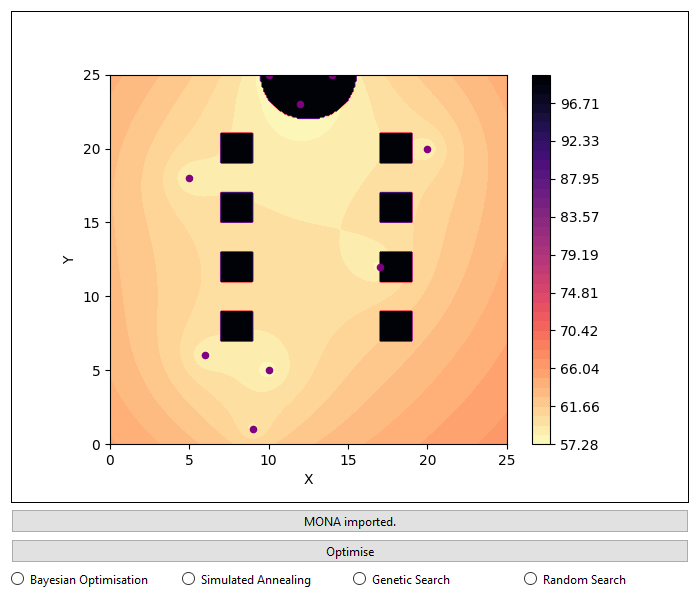
\includegraphics[scale=0.75]{graphics/gui}
		\caption{WNP GUI}
		\label{fig:gui}
		\end{figure}

		Figure \ref{fig:gui} shows a basic result. The floor plan can be seen along with the constraints, the points we are attempting to optimise around with their free space path loss shown as heat maps that gradually reduce as the distance increases.
		
	\subsection{Testing}
		\label{sec:software_testing}
		Below are some abbreviated test suites that describe the fulfilment of the objectives given in chapter \ref{sec:intro}.
		\subsubsection{User Acceptance}
			\label{sec:software_acceptance}
			User acceptance testing guarantees that the command line interface and the graphical user interface are working as expected. \\
			\begin{center}
				\small
				\begin{tabular}{| p{5cm} | p{1.5cm} | p{5cm}|}
				\hline
				\textbf{Test Description} & \textbf{Pass or Fail} & \textbf{Contribution} \\
				\hline
				CLI: The specified bounds file is imported and its properties are displayed. & Pass & Users can specify bounds files to import through command line arguments. \\
				\hline
				CLI: The optimisations are run and their outputs are displayed. & Pass & Users receive the output of the traditional and novel optimisation techniques. \\
				\hline
				GUI: Bounds files are imported and their layout is displayed. & Pass & Users are shown their bounds file as a heat map graph. \\
				\hline
				GUI: Optimisation techniques can be chosen and their result is displayed. & Pass & Users are shown the output of their chosen optimisation technique on the aforementioned heat map graph. \\
				\hline
				\end{tabular}
			\end{center}
				
		\subsubsection{Unit Testing}
			\label{sec:software_unit}
			The unit test suite exists to ensure that changes to the codebase do not adversely affect the running of the software. \\
			\begin{center}
				\small
				% \begin{longtable}{| p{5cm} | p{2cm} | p{2cm} |}
				% 	\hline
				% 	\textbf{Test Suite} & \textbf{Test Count} & \textbf{Tests Passed} \\
				% 	\hline
				% 	Bounds Test Suite & 10 & 10 \\
				% 	\hline
				% 	Search Test Suite & 4 & 4 \\
				% 	\hline
				% \end{longtable}
			\end{center}
	\section{Extensions and Open Questions}
	\label{sec:extensions}
	Whilst I've endeavoured to provide as many of the tools for the optimisation of two-dimensional node placement problems as possible, the world of optimisation is as vast as it is deep and so necessarily there is further work that could be done to enhance the software produced in this project.

	Additionally there are open questions that research into might prove fruitful in allowing for a more seamless experience in optimising node placement for novice users and developers alike. 

	\subsection{3D Space}
		\label{sec:extensions_3d} 
		The physical world is three-dimensional. A two-dimensional abstraction of the real world allows for a more convenient understanding of the problem but we lose an entire dimensions worth of data in doing so. Taking for one final time our museum example, the museum in question may have very tall ceilings. If a team of network engineers were to take the results of a two-dimensional optimisation at face value and place the wireless nodes on the ceiling, the free space path loss of the distance from the ceiling to the point they hope to cover is lost entirely.

		This would be fairly easy to incorporate into the existing optimisation library as long as further bounds were given as to the height of the environment. Visualisation of this space may be difficult using tools such as matplotlib. A 3D environment `explorer' that allows a user to change the camera angle at will may make this more understandable but would require a great deal of work.

	\subsection{Hyperparameter Optimisation}  
		\label{sec:extensions_hyperparameter}
		Both our genetic algorithm and simulated annealing implementations have some hard coded values that may result in substandard optimisation results. We could make use use of our existing optimisation algorithms to optimise these values for the best configuration of the techniques to best serve the individual scenarios given to the libraries. It would significantly increase the time to completion of the optimisation, but a two-layer process in which we attempt an optimisation of the chosen algorithm and then run that algorithm could lead to more optimal results.
		
	\subsection{Multiple Objectives} 
		\label{sec:extensions_multiple_objectives}
		Currently, our optimisation library only supports objective functions that return a single result. In order to evaluate the configuration of networks according to multiple objectives, work would have to be done into implementing multiple objective versions of our concerned algorithms. Such algorithms do exist \cite{demarco2009mogamesh}\cite{younis2020placementsurvey} but the process of determining superiority of configurations with multiple objectives can be difficult and is the subject of research\cite{yoo2007pareto}.
	
	\subsection{Network Simulation}
		\label{sec:extensions_network_sim}
		\subsubsection{FSPL Extensions}
			\label{sec:extensions_FSPL}
			Currently our free space path loss implementation does not account for whether the physical constraints, such as support columns or physical objects in which nodes cannot be placed, may impact the signal strength of a point on the other side. Increasing the degree of accuracy in this regard would also increase the complexity of the objective function evaluation but as has been noted, Bayesian optimisation is an optimal method for scenarios where the objective function is expensive to evaluate.
			
		\subsubsection{Mobile Sensors} 
			\label{sec:extensions_moving_sensors} 
			In many environments, such as an office, laptops and mobile devices are constantly moving. Some research has been done into predicting future movements of sensors that networks seek to cover. Dynamic node repositioning schemes\cite{younis2020placementsurvey} that seek to ensure the wireless mesh network remains a fully connected graph and that sensors (laptops and mobile devices in this case) are still covered. Routing protocols that find the most efficient path from a sensor to a base station also exist to support the repositioning of nodes with minimal interruption to performance\cite{akyildiza47wireless}.
		
	\section{Conclusion}
\label{sec:conclusion}

In this document we have introduced wireless sensor mesh networks and the importance of node placement in those networks. Having given a mathematical definition of the problem and a practical definition in the form of the indoor museum example and detailing how constraints may affect our placement of the nodes, we discuss various optimisation methods both traditional and novel, implement them and compare their performance. The features of the software utilising these methods have been demonstrated and comparisons of several different measures of performance have been carried out. Potential extensions to this document and the software have been discussed alongside questions left open.
\subsection{Contributions} 
	\label{sec:conclusion_contribs} 
	
		\begin{description}	
		
			\item[$\bullet$ A software library for the optimising of 2D node placement]\hfill
			
			This library is general enough to be used in any 2D node placement project and also easily modifiable to suit more specific needs.
			
			\item[$\bullet$ Software aiding the use of the optimisation library]\hfill
			
			For users who do not have a great deal of programming skill, this software works out of the box to interface with the library in an easy to understand way.
			
			\item[$\bullet$ This document]\hfill
						
			We review techniques and compare their usefulness in response to the growth of the number of dimensions and the complexity of the objective function (see chapter \ref{sec:problem}).
			
		\end{description}

	\bibliography{citations}
	\bibliographystyle{ieeetr}
	
\end{document}
